% FileName: ./pump.tex
% Generated by: AcuReport
% Date: Mon Jun 28 01:49:18 Iran Standard Time 2010
\documentclass[letterpaper,12pt]{article}
\usepackage{graphicx}
\usepackage{hyperref}
\usepackage[3D]{movie15}
\begin{document}
\hypersetup{pdfborder={0 0 0} }
\begin{center}

\includegraphics[scale=0.141998054627]{./Figures/AcusimLogo.png}
\end{center}
\vspace*{2.00mm}\hspace*{\fill}\\
\begin{center}
\Large{ \textsc{ Pump Analysis Performed by AcuSolve\\Pump }}\\
\end{center}
\vspace*{1.00mm}\hspace*{\fill}\\
\begin{center}
\large{ \textsc{ Dr. Farzin Shakib }}\\
\end{center}
\vspace*{1.00mm}\hspace*{\fill}\\
\begin{center}
ACUSIM Software, Inc.\\
\end{center}
\begin{center}
Mon Jun 28 13:49:24 2010\\
\end{center}
\vspace*{1.00mm}\hspace*{\fill}\\
\vfill
\begin{center}
\emph{ACUSIM Software, Inc. 2685 Marine Way, Suite 1421, Mountain View, California 94043}\\
\end{center}
\begin{center}
Tel: (650) 988-9700 Fax: (650) 988-9770 \href{mailto:info@acusim.com}{info@acusim.com} http://www.acusim.com\\
\end{center}
\vfill
\newpage
\clearpage
\tableofcontents
\vfill
\newpage
\clearpage
\section{Background}

Some background information.
\\
\vfill
\newpage
\clearpage
\section{Problem description}

The geometry is given in Figure \ref{fig:geom}.
\\
\begin{figure}[!h!tbp]
\begin{center}
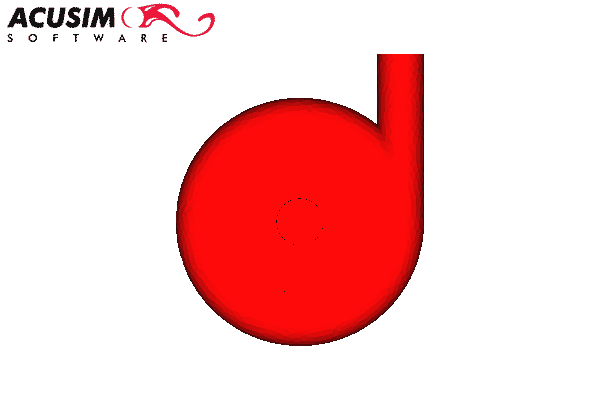
\includegraphics[scale=0.751879699248]{./Figures/Image_0.png}
\caption{\label{fig:geom}Geometry of the problem}
\end{center}
\end{figure}
\vfill
\newpage
\clearpage
\subsection{Mesh}

The geometry is given in Figure \ref{fig:mesh}.
\\
\begin{figure}[!h!tbp]
\begin{center}
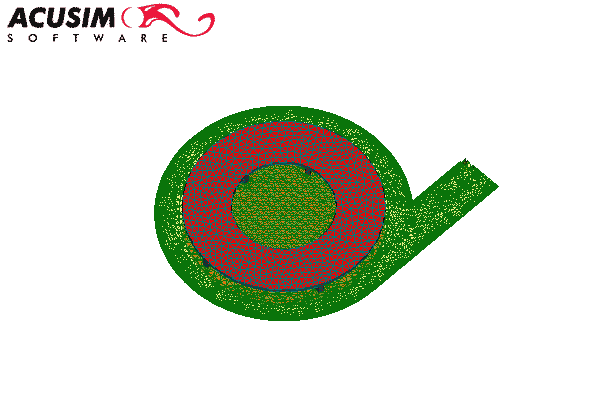
\includegraphics[scale=0.751879699248]{./Figures/Image_1.png}
\caption{\label{fig:mesh}Geometry of the mesh}
\end{center}
\end{figure}
\vfill
\newpage
\clearpage
\subsection{Solver Settings}
Material model is given by:\\\\
Material Model for Fluid 'Water'\\
\begin{itemize}
\item{\emph{Density Model}}

\begin{itemize}
\item{\emph{Type = Constant}}

\item{\emph{Density = 1000.0}}

\item{\emph{Isothermal compressibility = 0.0}}

\end{itemize}
\item{\emph{Viscosity Model}}

\begin{itemize}
\item{\emph{Type = Constant}}

\item{\emph{Viscosity = 0.001}}

\item{\emph{Multiplier function = None}}

\end{itemize}
\end{itemize}
Rotational speed is 10\\
\begin{figure}[!h!tbp]
\begin{center}
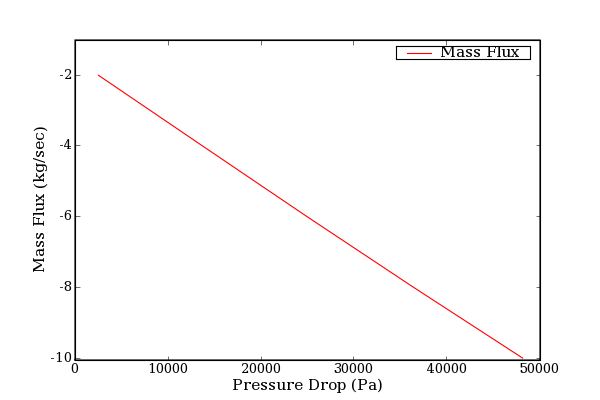
\includegraphics[scale=0.751879699248]{./Figures/plot_1.png}
\caption{\label{fig:mp}Fan performance}
\end{center}
\end{figure}
\begin{table}[!h!tbp]
\begin{center}
\begin{tabular}{| l | l | }
\hline
Pressure Drop (Pa) & Mass Flux (Kg/sec) \\
\hline
2506.57 & -2.00 \\
\hline
13707.15 & -4.00 \\
\hline
24949.46 & -6.00 \\
\hline
36406.80 & -8.00 \\
\hline
48129.20 & -10.00 \\
\hline
\end{tabular}
\caption{\label{tab:mp}
Fan performance}
\end{center}
\end{table}

The fan performance curve is given in Figure \ref{fig:mp} and Table
\ref{tab:mp}
\\
\vfill
\newpage
\clearpage
\section{Results}

The results are given in the following figures.
\\

The pressure distribution are shown in the following figures.
\\
\begin{figure}[!h!tbp]
\begin{center}
\begin{tabular}{ p{7cm} p{7cm} }
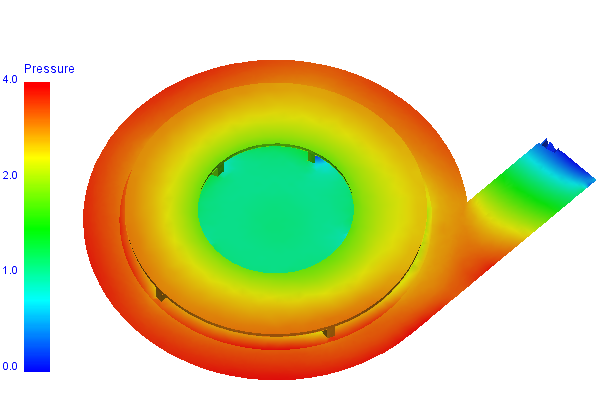
\includegraphics[scale=0.263157894737]{./Figures/Image_2.png}
 & 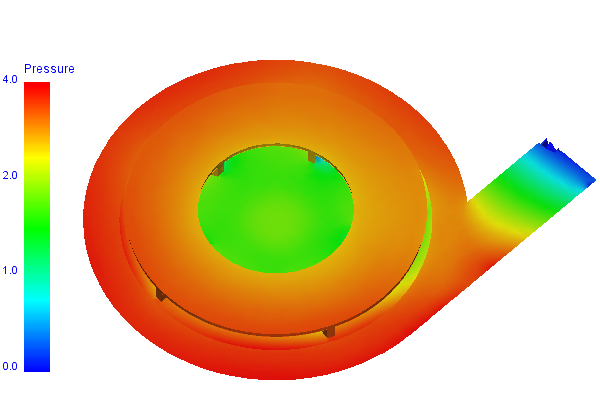
\includegraphics[scale=0.263157894737]{./Figures/Image_3.png}
 \\ a. mass flux = -2 & b. mass flux = -4 \\
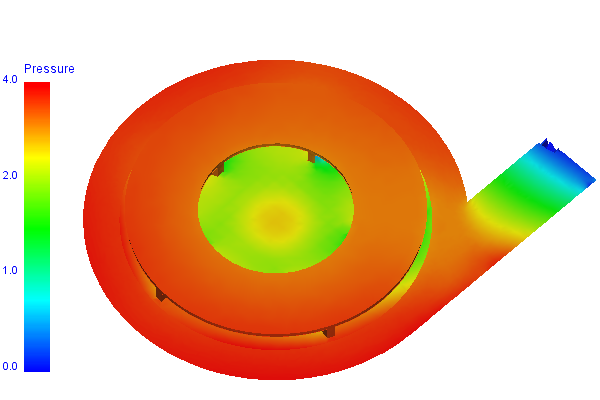
\includegraphics[scale=0.263157894737]{./Figures/Image_4.png}
 & 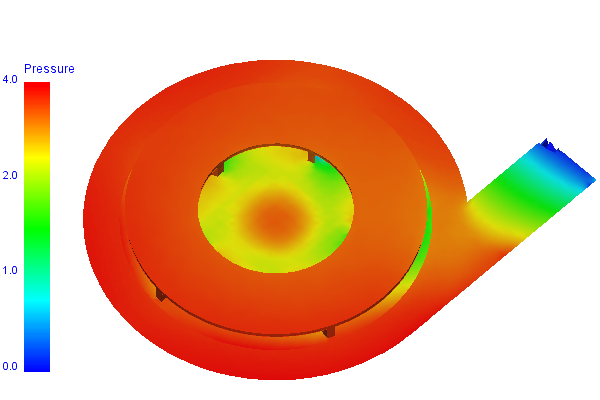
\includegraphics[scale=0.263157894737]{./Figures/Image_5.png}
 \\ c. mass flux = -6 & d. mass flux = -8 \\
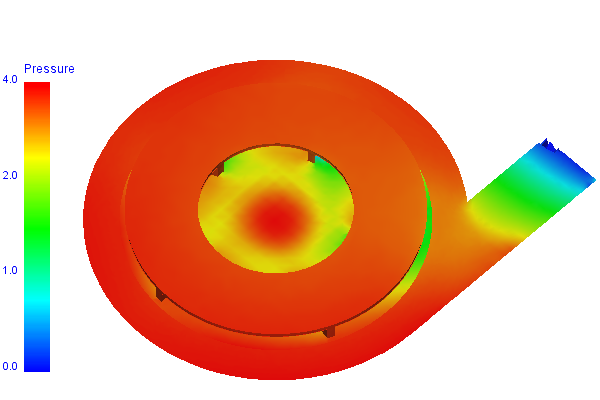
\includegraphics[scale=0.263157894737]{./Figures/Image_6.png}
 &  \\ e. mass flux = -10 &  \\
\end{tabular}
\caption{\label{fig:pres}
Pressure contour on center plane}
\end{center}
\end{figure}
\vfill
\newpage
\clearpage

The velocity distribution are shown in the following figures.
\\
\begin{figure}[!h!tbp]
\begin{center}
\begin{tabular}{ c c }
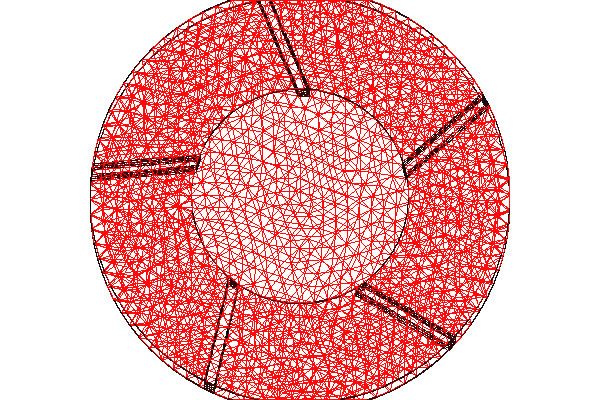
\includegraphics[scale=0.263157894737]{./Figures/Image_7.png}
 & 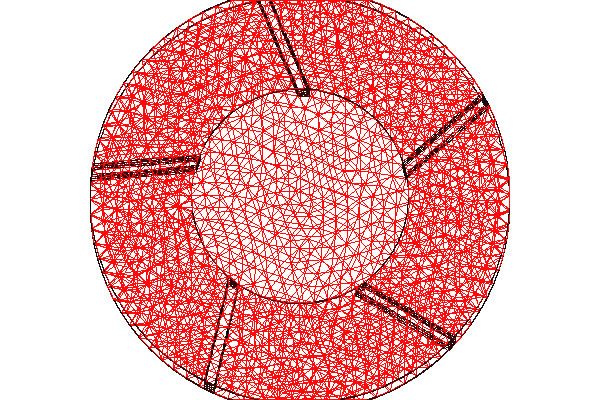
\includegraphics[scale=0.263157894737]{./Figures/Image_8.png}
 \\ a. mass flux = -2 & b. mass flux = -4 \\
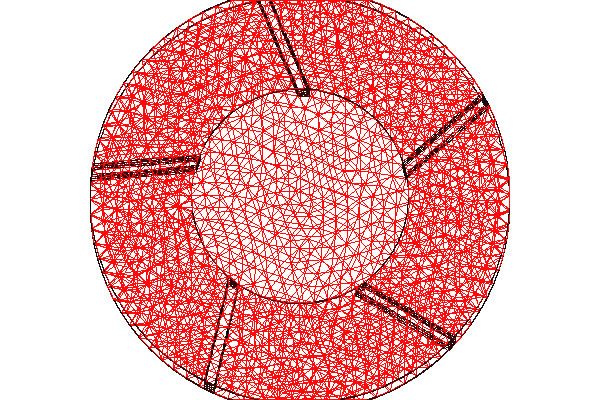
\includegraphics[scale=0.263157894737]{./Figures/Image_9.png}
 & 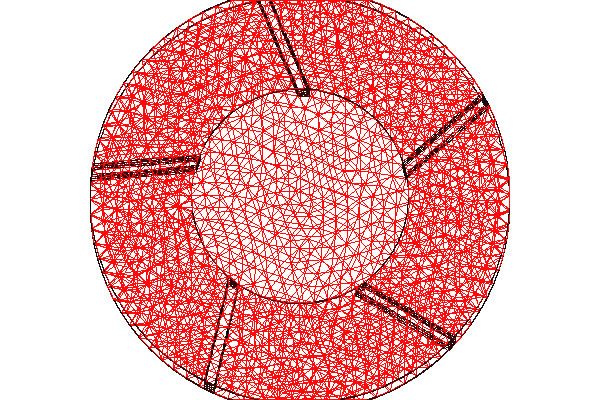
\includegraphics[scale=0.263157894737]{./Figures/Image_10.png}
 \\ c. mass flux = -6 & d. mass flux = -8 \\
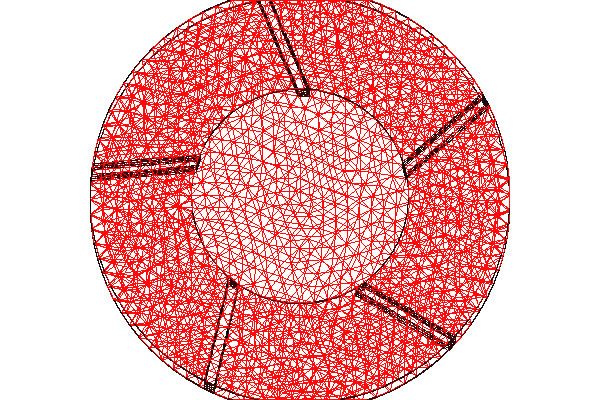
\includegraphics[scale=0.263157894737]{./Figures/Image_11.png}
 &  \\ e. mass flux = -10 &  \\
\end{tabular}
\caption{\label{fig:vel}
Velocity vector on center plane}
\end{center}
\end{figure}
\vfill
\newpage
\clearpage

Several samples of clipping are shown in the following figures.
\\
\begin{figure}[!h!tbp]
\begin{center}
\begin{tabular}{ c c }

\includegraphics[scale=0.263157894737]{./Figures/Fully-TransparentUPClipPlane.png}
 & 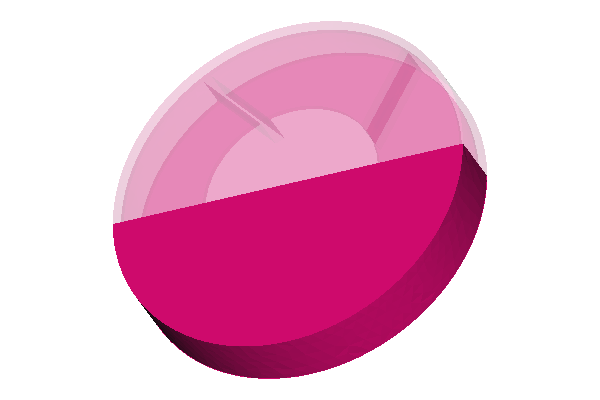
\includegraphics[scale=0.263157894737]{./Figures/90-TransparentDownClipPlane.png}
 \\ Fully-Transparent 'Up' Clip Plane & 90\%-Transparent 'Down' Clip Plane \\

\includegraphics[scale=0.263157894737]{./Figures/Fully-TransparentMaxClipBox.png}
 & 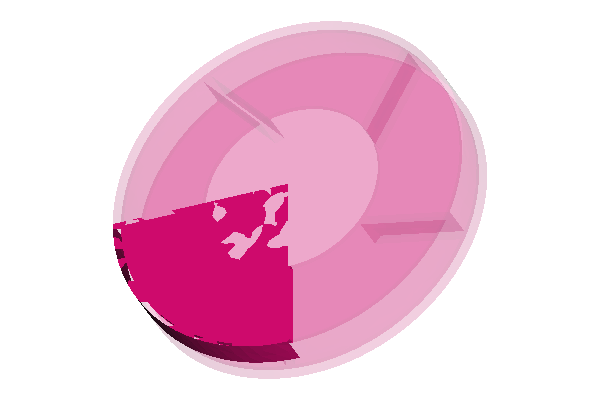
\includegraphics[scale=0.263157894737]{./Figures/90-TransparentMaxClipBox.png}
 \\ Fully-Transparent 'Max' Clip Box & 90\%-Transparent 'Max' Clip Box \\
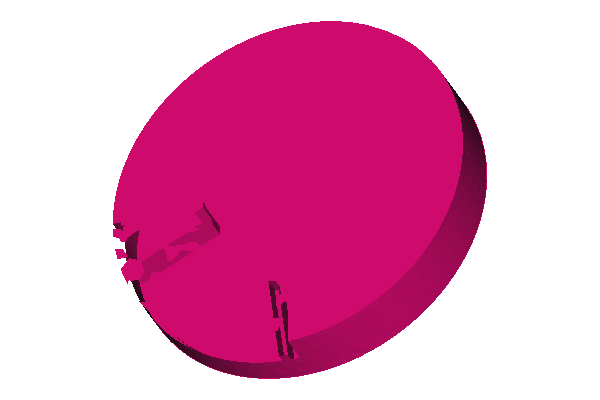
\includegraphics[scale=0.263157894737]{./Figures/Fully-TransparentMinClipBox.png}
 & 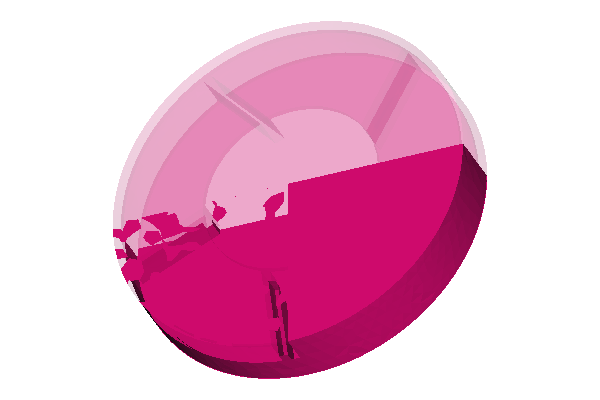
\includegraphics[scale=0.263157894737]{./Figures/90-TransparentPrepMinClipBox.png}
 \\ Fully-Transparent 'Min' Clip Box & 90\%-Transparent [Prep by a Clip-Plane] 'Min' Clip Box \\
\end{tabular}
\caption{\label{fig:clp}
Clipping Samples}
\end{center}
\end{figure}
\vfill
\newpage
\clearpage
\section{Conclusions}

Some conclusion goes here
\\
\end{document}
